% !TeX program = pdflatex
\documentclass{beamer}
\usetheme{Madrid}
\usecolortheme{default}

\usepackage[utf8]{inputenc}
\usepackage[T1]{fontenc}
\usepackage{amsmath, amssymb}
\usepackage{graphicx}
\usepackage{booktabs}
\usepackage{siunitx}
\usepackage{verbatim}
\usepackage{tikz}



\title[Conversores A/D]{Conversores Analógico-Digitais (A/D): Técnicas de Construção, Estruturas e Aplicações}
\subtitle{Instrumentação Eletrônica}
\author[GCET521]{%
    \textbf{Discentes:} Lucas Souza de Castro \\
    Claudio Roberto Silveira Eloy Junior\\ 
    Ricardo Teixeira dos Santos
}
\institute[UFRB]{Universidade Federal do Recôncavo da Bahia}
\date{Cruz das Almas, 2026}  % Data para o rodapé

\begin{document}

\setbeamertemplate{background}{%
    \begin{tikzpicture}[overlay, remember picture]
        \node[opacity=0.10] at ([xshift=-2.0cm, yshift=1.2cm] current page.south east) { % Ajuste a opacidade aqui
            
\includegraphics[width=0.3\paperwidth]{figures/ufrb.png} % Ajuste o tamanho e o nome do arquivo
        };
    \end{tikzpicture}%
}

\begin{frame}[plain] % 'plain' remove cabeçalho/rodapé dessa página (opcional)
    \vfill
    \begin{center}
        \begin{beamercolorbox}[sep=8pt,center,rounded=true,shadow=true]{title}
            \usebeamerfont{title}\inserttitle\par
            \ifx\insertsubtitle\empty\else
                \vskip0.5em
                {\usebeamerfont{subtitle}\usebeamercolor[fg]{subtitle}\insertsubtitle\par}
            \fi
        \end{beamercolorbox}
        \vskip1em
        
        {\usebeamerfont{institute}\usebeamercolor[fg]{institute}\Large\insertinstitute\par}
        \vskip1.5em
        
        \begin{beamercolorbox}[sep=8pt,center]{author}
            \usebeamerfont{author}\insertauthor\par
        \end{beamercolorbox}
        \vskip1em
        
        {\small \textbf{Prof. Orientador:} Nilton Cardoso da Silva\par}
        
    \end{center}
    \vfill
\end{frame}
% ===================== SLIDE 2: SUMÁRIO GERAL =====================
\begin{frame}{Sumário}
    \small % Reduz a fonte para ganhar espaço vertical
    \begin{columns}[T]
        \begin{column}{0.48\textwidth} % Margem de segurança à esquerda
            \textbf{Parte 1: Fundamentos e Amostragem} \hfill \textcolor{gray}{}
            \begin{itemize}
                \setlength{\itemsep}{0pt}      % Remove espaços extras entre itens
                \setlength{\parskip}{0pt}
                \item Introdução e Motivação
                \item Sinais Analógicos vs. Digitais
                \item Processo de Conversão: Amostragem
                \item Teorema de Nyquist
                \item Aliasing e Filtros Anti-Aliasing
            \end{itemize}
            
            \vspace{0.1cm} % Espaço mínimo entre as partes
            \textbf{Parte 2: Arquiteturas Clássicas} \hfill \textcolor{gray}{}
            \begin{itemize}
                \setlength{\itemsep}{0pt}
                \setlength{\parskip}{0pt}
                \item Conversor Flash (Paralelo)
                \item SAR (Aproximações Sucessivas) % Nome encurtado para caber melhor
                \item Sigma-Delta ($\Sigma\Delta$)
            \end{itemize}
        \end{column}
        
        \begin{column}{0.48\textwidth} % Margem de segurança à direita
            \textbf{Parte 3: Comparação e Aplicações} \hfill \textcolor{gray}{}
            \begin{itemize}
                \setlength{\itemsep}{0pt}
                \setlength{\parskip}{0pt}
                \item Resolução, Velocidade e Precisão
                \item Comparativo entre Arquiteturas
                \item Aplicações em Sistemas Embarcados
                \item Automação Industrial e Instrumentação
                \item Integração com Sensores e MCUs % Abreviação para ganhar espaço
                \item Conclusões Finais
            \end{itemize}
        \end{column}
    \end{columns}
\end{frame}

% ============================================================
% ===================== PARTE 1: LUCAS ======================
% ============================================================
\begin{frame}{Fundamentos da Conversão A/D}
    A maioria dos fenômenos físicos (temperatura, pressão, som, luz) são analógicos (contínuos no tempo e amplitude).
    Sistemas digitais (microcontroladores, DSPs) processam informações como dígitos binários (0 e 1).

    \begin{columns}[onlytextwidth] 
        \begin{column}{0.48\textwidth} % Coluna da esquerda
            \centering
            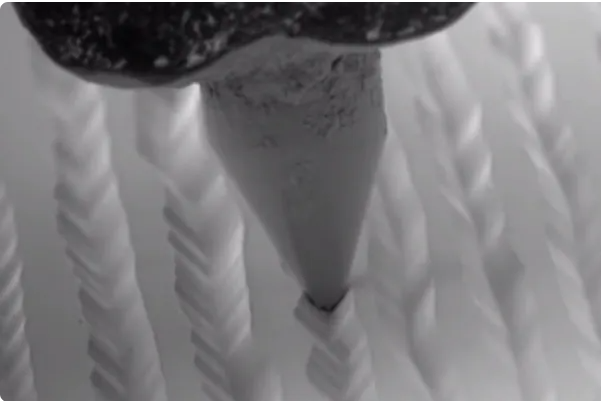
\includegraphics[width=\linewidth]{figures/vinil.png}
            \smallskip
            {\small \textbf{Figura 1:} Sulcos do disco de vinil}
        \end{column}
        \hfill 
        \begin{column}{0.48\textwidth} % Coluna da direita
            \centering
            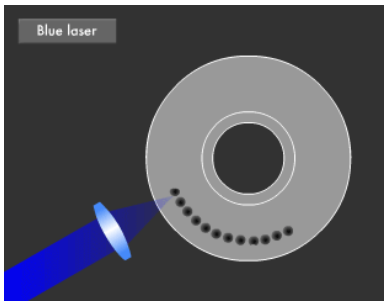
\includegraphics[width=\linewidth]{figures/cd.png}
            \smallskip
            {\small \textbf{Figura 2:} pits  de um CD}
        \end{column}
    \end{columns}

\end{frame}

\begin{frame}{Definições: Sinais Analógicos vs. Digitais}
    \begin{columns}[c]
        \begin{column}{0.5\textwidth}
            \textbf{Analógico}
            \begin{itemize}
                \item Contínuo no tempo % valores infinitos entre dois pontos
                \item Contínuo em amplitude
                \item Resolução infinita % Teoricamente, não perde detalhes (como a nuance mais sutil de um violino)
            \end{itemize}
        \end{column}
        \begin{column}{0.5\textwidth}
            \textbf{Digital}
            \begin{itemize}
                \item Discreto no tempo
                \item Discreto em amplitude
                \item Resolução finita %definida pela taxa de amostragem e profundidade de bits
            \end{itemize}
        \end{column}
    \end{columns}
    \vspace{0.3cm}
    \begin{figure}
    \centering
    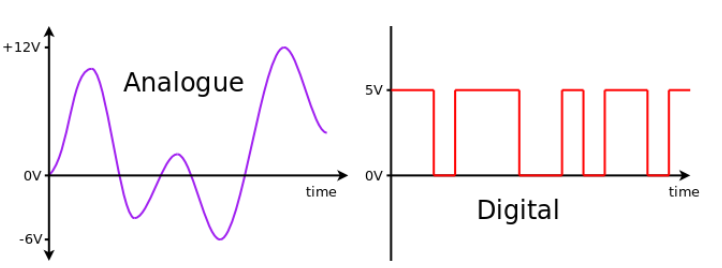
\includegraphics[width=0.8\textwidth]{figures/fig1.png}
    \par
    {\small \textbf{Figura 3:} Sinal analógico e Sinal digital}
\end{figure}
\end{frame}

\begin{frame}{Processo de Conversão A/D: As 3 Etapas}
    \begin{enumerate}
        \item \textbf{Amostragem (Sampling):} Capturar o valor do sinal em instantes discretos de tempo.
        \item \textbf{Quantização:} Arredondar a amplitude para um nível finito (aproximação).
        \item \textbf{Codificação:} Representar o nível quantizado em binário (bits).
    \end{enumerate}
    \vspace{0.3cm}
    \begin{figure}
        \centering
        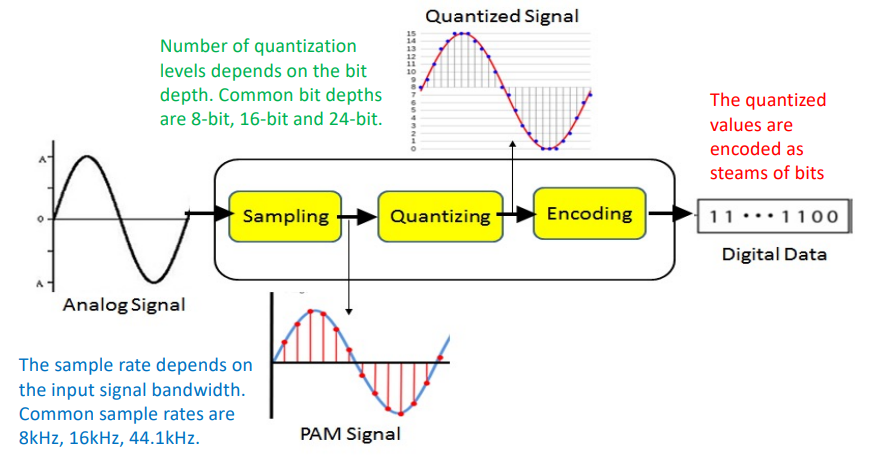
\includegraphics[width=0.7\textwidth]{figures/sample.png}
        \par
        {\small \textbf{Figura 4:} Diagrama de blocos do processo de conversão}
    \end{figure}
\end{frame}

\begin{frame}{Amostragem: O Coração da Conversão}
    \begin{itemize}
        \item O sinal é \textbf{amostrado} (lido) em intervalos regulares $T_s$ (período de amostragem).
        \item $f_s = 1/T_s$ é a \textbf{frequência de amostragem}.
    \end{itemize}
    \begin{block}{Teorema de Nyquist-Shannon}
        Para recuperar o sinal sem perdas, a frequência de amostragem deve ser \textbf{pelo menos o dobro} da maior frequência presente no sinal:
        \[
            f_s \ge 2 \cdot f_{max}
        \]
        Onde $f_{max}$ é a frequência máxima do sinal (largura de banda).
    \end{block}
\end{frame}

\begin{frame}{Aliasing: O Efeito Indesejado}
    \begin{block}{O que é Aliasing?}
        Quando $f_s < 2 f_{max}$, ocorre a \textbf{sobreposição espectral}: altas frequências "se disfarçam" de baixas frequências.
    \end{block}

            \centering
            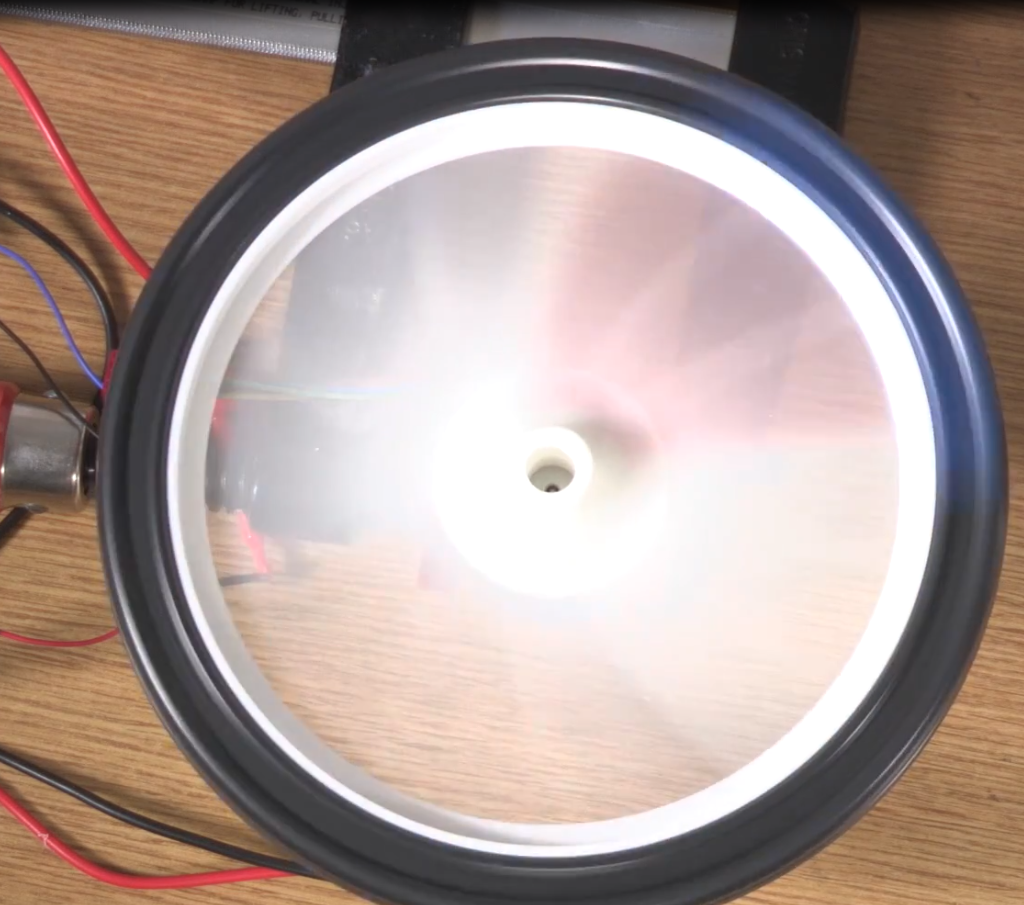
\includegraphics[width=0.4\textwidth]{figures/video.png}
            \par
            {\small \textbf{Figura 5:} imagem do efeito de aliasing em 2min e 40s}
\end{frame}

\begin{frame}{Filtro Anti-Aliasing}
    \begin{itemize}
        \item Para evitar o aliasing, usa-se um \textbf{filtro passa-baixas} antes do conversor A/D.
        \item O filtro atenua todas as frequências acima de $f_s/2$ (frequência de Nyquist).
    \end{itemize}
    \begin{figure}
        \centering
        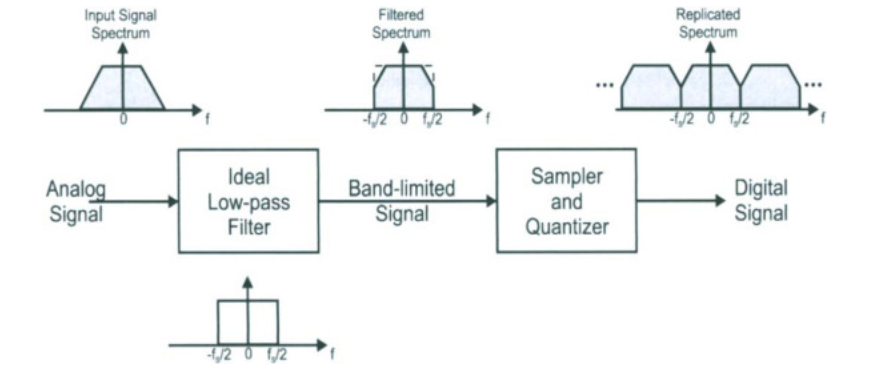
\includegraphics[width=0.7\textwidth]{figures/powpass.png}
        \par
        {\small \textbf{Figura 6:} diagrama de blocos com filtro pb}
    \end{figure}
    \vspace{0.2cm}
\end{frame}

% ============================================================
% ===================== PARTE 2: CLÁUDIO =====================
% ============================================================

\begin{frame}{Parte 2: Arquiteturas de Conversores A/D}
    \begin{center}
        \Large{\textbf{Flash, SAR e Sigma-Delta}} \\
        \vspace{0.5cm}
        \textit{Apresentador: Claudio Roberto Silveira Eloy Junior}
    \end{center}
\end{frame}

\begin{frame}{Arquitetura Flash (Paralelo)}
    \begin{block}{Princípio}
        Utiliza um \textbf{banco de comparadores} ligados em paralelo, cada um com uma referência de tensão diferente (gerada por um divisor resistivo).
    \end{block}
    \begin{figure}
        \centering
        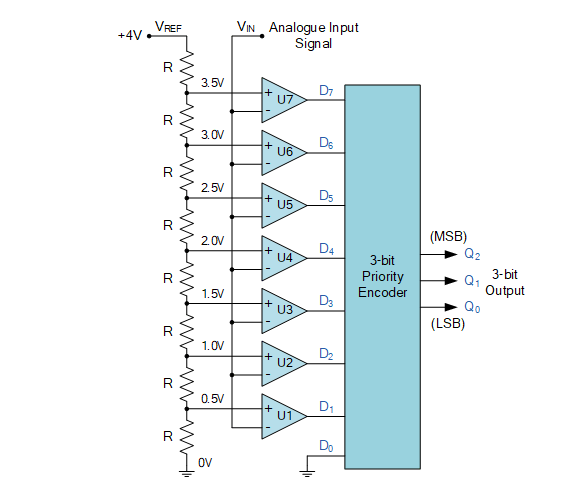
\includegraphics[width=0.5\textwidth]{figures/conv-3bits.png}
        \fbox{\small Figura: Estrutura básica de um conversor Flash de 3 bits}
    \end{figure}
\end{frame}

\begin{frame}{Arquiteteura Flash: Vantagens e Desvantagens}
    \begin{columns}[t]
        \begin{column}{0.5\textwidth}
            \textbf{Vantagens}
            \begin{itemize}
                \item \textcolor{green}{Muito rápido} (operação paralela)
                \item Latência de 1 ciclo de clock
            \end{itemize}
        \end{column}
        \begin{column}{0.5\textwidth}
            \textbf{Desvantagens}
            \begin{itemize}
                \item \textcolor{red}{Alto custo} e consumo para alta resolução
                \item Precisa de $2^n - 1$ comparadores para $n$ bits
            \end{itemize}
        \end{column}
    \end{columns}
\end{frame}

\begin{frame}{Arquitetura SAR (Aproximações Sucessivas)}
    \begin{block}{Princípio de Funcionamento}
        Funciona como uma \textbf{balança digital}. O SAR testa um bit por vez, do MSB ao LSB, ajustando um DAC interno até que a saída do DAC iguale a entrada analógica.
    \end{block}
    \begin{figure}
        \centering
         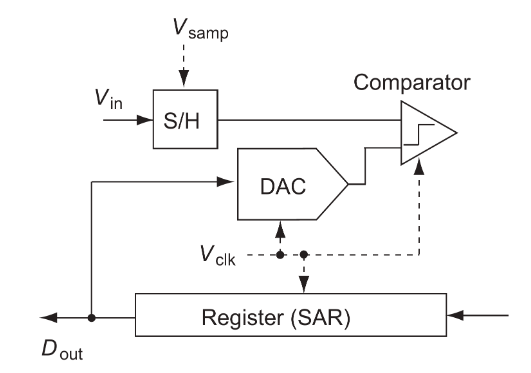
\includegraphics[width=0.5\textwidth]{figures/Diagrama_SAR.png}
        \fbox{\small Figura: Diagrama de blocos de um conversor SAR}
    \end{figure}
\end{frame}

\begin{frame}{Arquitetura SAR: Vantagens e Desvantagens}
    \begin{columns}[t]
        \begin{column}{0.5\textwidth}
            \textbf{Vantagens}
            \begin{itemize}
                \item \textcolor{green}{Boa relação custo/velocidade}
                \item \textcolor{green}{Baixo consumo de energia}
                \item Resolução típica de 8 a 16 bits
            \end{itemize}
        \end{column}
        \begin{column}{0.5\textwidth}
            \textbf{Desvantagens}
            \begin{itemize}
                \item \textcolor{red}{Velocidade limitada} (requer $n$ ciclos de clock)
                \item Sensível a ruídos no comparador
            \end{itemize}
        \end{column}
    \end{columns}
\end{frame}

\begin{frame}{Arquitetura Sigma-Delta ($\Sigma\Delta$)}
    \begin{block}{Princípio de Funcionamento}
        Utiliza \textbf{modulação sigma-delta} (sobreamostragem e moldagem de ruído) para alcançar altíssima resolução.
    \end{block}
    \begin{figure}
        \centering
        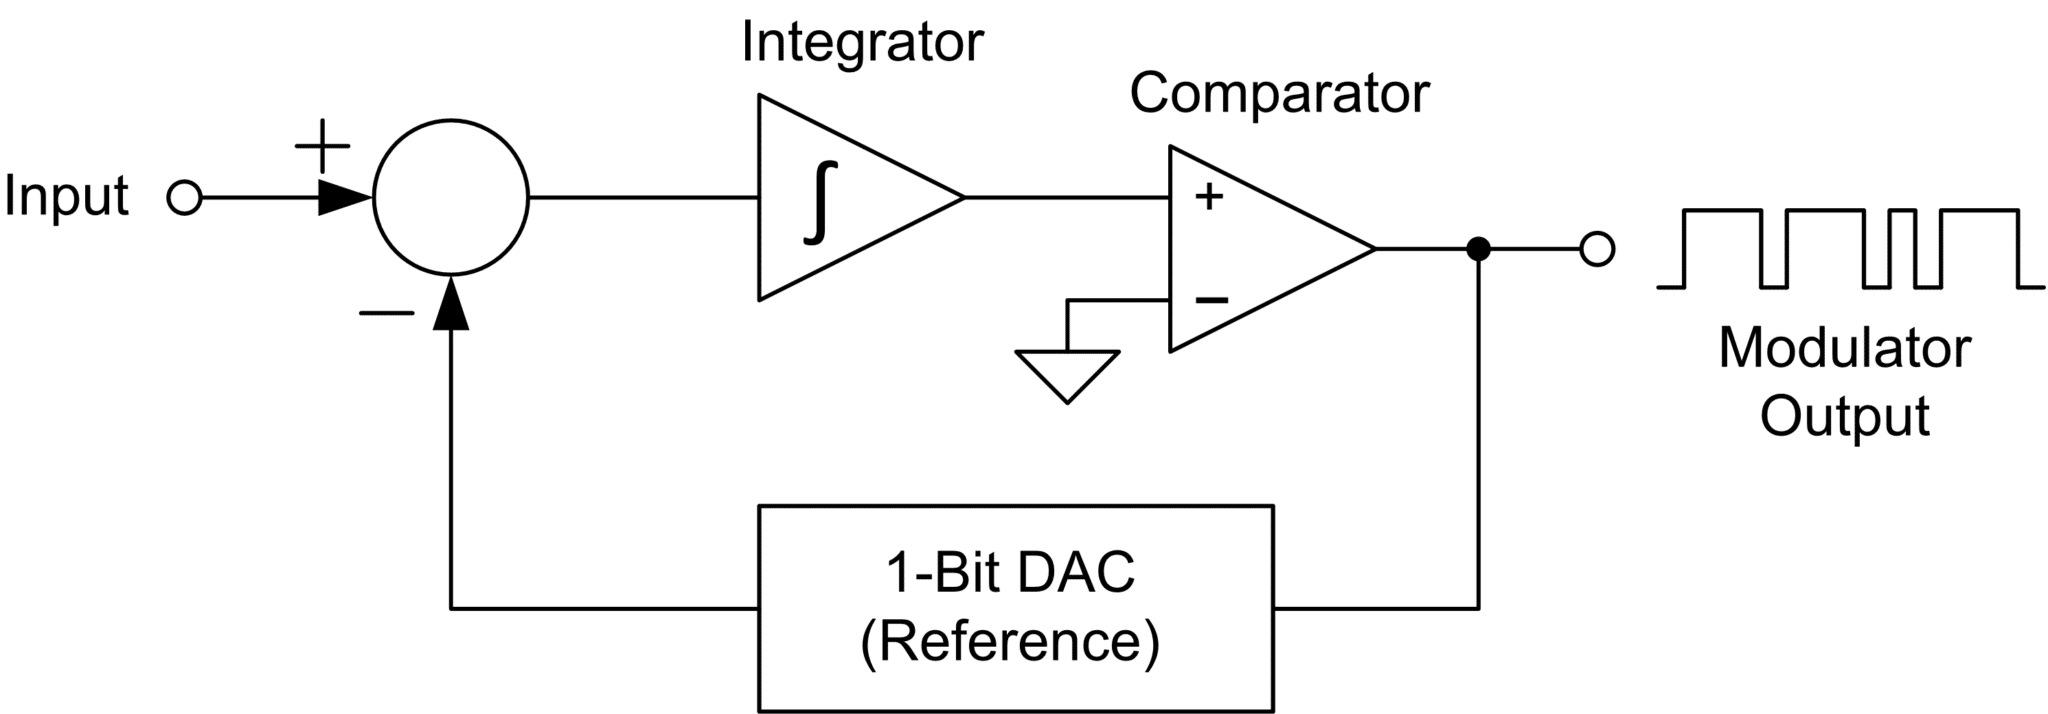
\includegraphics[width=0.6\textwidth]{figures/delta-sigma.png}
        \fbox{\tiny Figura: Estrutura básica de um modulador Sigma-Delta de 1ª ordem}
    \end{figure}
    \begin{columns}[t]
        \begin{column}{0.5\textwidth}
            \textbf{\small Vantagens}
            \begin{itemize}
                \item \textcolor{green}{\footnotesize Altíssima resolução} (16 a 24 bits){}
                \item \textcolor{green}{\footnotesize Excelente linearidade}
                \item {\footnotesize Baixo custo para alta resolução}
            \end{itemize}
        \end{column}
        \begin{column}{0.5\textwidth}
            \textbf{\small Desvantagens}
            \begin{itemize}
                \item \textcolor{red}{\footnotesize Velocidade baixa} (devido à sobreamostragem)
                \item \textcolor{red}{\footnotesize Latência alta} (vários ciclos)
            \end{itemize}
        \end{column}
    \end{columns}
\end{frame}

\begin{frame}{Comparação Visual das Arquiteturas}
    \begin{table}
        \centering
        \footnotesize % Diminui a fonte para caber
        \setlength{\tabcolsep}{4pt} % Estreita o espaço entre colunas
        \begin{tabular}{lccc}
            \toprule
            \textbf{Característica} & \textbf{Flash} & \textbf{SAR} & \textbf{$\Sigma\Delta$} \\
            \midrule
            Velocidade & \textcolor{blue}{Muito Alta} & \textcolor{orange}{Média} & \textcolor{red}{Baixa} \\
            Resolução & \textcolor{red}{Baixa (8 bits)} & \textcolor{orange}{Média (12-16 bits)} & \textcolor{blue}{Alta (16-24 bits)} \\
            Custo & Alto & Médio & Médio/Baixo \\
            Consumo & Alto & Baixo & Médio \\
            Aplicação & Vídeo, Radar & Controle, Áudio & Áudio, Instrumentação \\
            \bottomrule
        \end{tabular}
        \caption{Comparação resumida entre as arquiteturas.}
    \end{table}
\end{frame}

\begin{frame}{Resumo da Parte 2}
    \begin{itemize}
        \item \textbf{Flash:} Máxima velocidade, baixa resolução, alto custo.
        \item \textbf{SAR:} Equilíbrio entre velocidade, resolução e custo. Muito utilizado em microcontroladores.
        \item \textbf{Sigma-Delta:} Máxima resolução, baixa velocidade, ideal para sinais de baixa frequência (áudio, sensores de precisão).
    \end{itemize}
    \vspace{0.5cm}
    \begin{center}
        \textit{"Na terceira parte, vamos explorar como escolher o conversor certo e onde eles são aplicados."}
    \end{center}
\end{frame}

% ============================================================
% ===================== PARTE 3: RICARDO =====================
% ============================================================

\begin{frame}{Parte 3: Aplicações e Critérios de Escolha}
    \begin{center}
        \Large{\textbf{Comparação e Aplicações}} \\
        \vspace{0.5cm}
        \textit{Apresentador: Ricardo Teixeira dos Santos}
    \end{center}
\end{frame}

\begin{frame}{Resolução, Velocidade e Precisão}
	
	\begin{block}{Resolução}
		\begin{itemize}
			\item Define o menor incremento de tensão detectável (LSB).
			\item Um ADC de $n$ bits possui $2^n$ níveis de quantização.
			\item Quanto maior a resolução, menor o erro de quantização.
		\end{itemize}
		\[
		LSB=\frac{V_{ref}}{2^n}
		\]
	\end{block}
	
	\begin{block}{Velocidade}
		\small
		\begin{itemize}
			\item Determinada pela taxa de amostragem ($f_s$).
			\item Quanto maior a velocidade, maior a largura de banda do sinal.
		\end{itemize}
	\end{block}
	
	\begin{block}{Precisão}
		\small
		
		Depende da resolução e dos erros do conversor.
		
		\begin{columns}[T]
			\column{0.24\textwidth}
			\begin{itemize}
				\item Offset
			\end{itemize}
			\column{0.24\textwidth}
			\begin{itemize}
				\item Ganho
			\end{itemize}
			\column{0.24\textwidth}
			\begin{itemize}
				\item INL
			\end{itemize}
			\column{0.24\textwidth}
			\begin{itemize}
				\item DNL
			\end{itemize}
		\end{columns}
		
	\end{block}
\end{frame}


\begin{frame}{Comparativo entre Arquiteturas}
	
	\begin{table}
		\centering
		\footnotesize
		\begin{tabular}{lcccc}
			\toprule
			\textbf{Arquitetura} & \textbf{Velocidade} & \textbf{Resolução} & \textbf{Consumo} & \textbf{Aplicação} \\
			\midrule
			Flash & Muito alta & Baixa & Alto & Radar, Vídeo \\
			SAR & Média/Alta & Média & Baixo & Sistemas Embarcados \\
			$\Sigma\Delta$ & Baixa & Muito alta & Médio & Instrumentação, Áudio \\
			\bottomrule
		\end{tabular}
	\end{table}
	
	\vspace{0.3cm}
	
	\begin{alertblock}{Conclusão}
		Não existe um ADC melhor, mas sim o mais adequado para cada aplicação.
	\end{alertblock}
	
\end{frame}

\begin{frame}{Aplicações em Sistemas Embarcados}
	
	\begin{itemize}
		\item Microcontroladores possuem ADCs integrados, geralmente do tipo SAR.
		\item Conversão de sinais analógicos provenientes de sensores.
		\item Monitoramento de bateria e alimentação.
		\item Controle de motores e robótica.
		\item Sistemas IoT e automotivos.
	\end{itemize}
	
	\vspace{0.3cm}
	
	\begin{block}{Exemplos}
		\begin{itemize}
			\item Arduino Uno -- ADC SAR de 10 bits.
			\item ESP32 -- ADC SAR de 12 bits.
			\item STM32 -- ADC SAR de 12 ou 16 bits.
		\end{itemize}
	\end{block}
	
\end{frame}

\begin{frame}{Automação Industrial e Instrumentação}
	
	\begin{columns}
		
		\column{0.48\textwidth}
		
		\textbf{Automação Industrial}
		
		\begin{itemize}
			\item Leitura de sensores industriais.
			\item Controle PID.
			\item Monitoramento de processos.
			\item Entradas analógicas de CLPs.
			\item Sinais de 0--10 V e 4--20 mA.
		\end{itemize}
		
		\column{0.48\textwidth}
		
		\textbf{Instrumentação}
		
		\begin{itemize}
			\item Multímetros digitais.
			\item Osciloscópios.
			\item Sistemas DAQ.
			\item Equipamentos biomédicos.
			\item Instrumentos de alta precisão.
		\end{itemize}
		
	\end{columns}
	
	\vspace{0.3cm}
	
	\begin{alertblock}{Importante}
		Quanto maior a precisão exigida, maior deve ser a resolução do conversor.
	\end{alertblock}
	
\end{frame}

\begin{frame}{Integração com Sensores e Microcontroladores}
	
	\begin{center}
		
		\Large
		
		Sensor
		
		$\downarrow$
		
		Condicionamento do sinal
		
		(Filtro / Amplificador)
		
		$\downarrow$
		
		Conversor A/D
		
		$\downarrow$
		
		Microcontrolador
		
		$\downarrow$
		
		Processamento e Controle
		
		$\downarrow$
		
		Display / Comunicação / Atuador
		
	\end{center}
	
	\vspace{0.4cm}
	
	\begin{itemize}
		\item Sensores fornecem sinais analógicos.
		\item O ADC converte esses sinais para o domínio digital.
		\item O microcontrolador processa as informações e executa ações.
	\end{itemize}
	
\end{frame}

\begin{frame}{Qual Conversor Escolher?}
	
	\begin{table}
		\centering
		\begin{tabular}{ll}
			\toprule
			\textbf{Prioridade} & \textbf{Arquitetura Recomendada} \\
			\midrule
			Máxima velocidade & Flash \\
			Baixo consumo & SAR \\
			Alta resolução & $\Sigma\Delta$ \\
			Sistemas embarcados & SAR \\
			Instrumentação & $\Sigma\Delta$ \\
			Vídeo e Radar & Flash \\
			\bottomrule
		\end{tabular}
	\end{table}
	
	\vspace{0.5cm}
	
	\begin{block}{Mensagem Final}
		A escolha de um conversor A/D depende do equilíbrio entre velocidade, resolução, consumo de energia e custo da aplicação.
	\end{block}
	
\end{frame}

\begin{frame}{Conclusões Finais}
    \begin{itemize}
        \item A escolha do conversor A/D é uma decisão de \textbf{engenharia} que envolve um \textit{trade-off} entre velocidade, resolução, custo e consumo.
        \item \textbf{Flash:} Velocidade extrema, baixa resolução.
        \item \textbf{SAR:} A escolha mais versátil para a maioria das aplicações embarcadas.
        \item \textbf{Sigma-Delta:} A escolha para aplicações de alta precisão e baixa frequência.
        \item A conversão A/D é um pilar fundamental da eletrônica moderna, presente desde um simples termômetro digital até sistemas de comunicação e controle de processos.
    \end{itemize}
\end{frame}

\begin{frame}{Referências Bibliográficas}
    \begin{thebibliography}{9}
        \bibitem{sedra} SEDRA, A. S.; SMITH, K. C. \textit{Microelectronic Circuits}. 7. ed. Oxford University Press, 2014.
        \bibitem{malvino} MALVINO, A. P.; BATES, D. J. \textit{Eletrônica}. 7. ed. McGraw-Hill, 2017.
        \bibitem{datasheets} Datasheets: Analog Devices, Texas Instruments (ADC0804, ADS1115, etc.).
        \bibitem{artigo} BAKER, Bonnie. \textit{How to Select the Right ADC for Your Application}. Analog Devices, AN-283.
    \end{thebibliography}
\end{frame}

\begin{frame}{}
    \begin{center}
        \Huge{\textbf{Obrigado!}}
        \vspace{1cm}
        \Large{Dúvidas?}
    \end{center}
\end{frame}

\end{document}